
\title[Agile]{Agile}
\date{}
\author[Pepe Doval]{}
\institute{}

\section{Agile}
\label{sec:Agile}

\usebackgroundtemplate{}
\begin{frame}
  \titlepage
\end{frame}

\usebackgroundtemplate{%
  \tikz[overlay,remember picture] 
  \node[opacity=0.3 , at=(current page.south east),anchor=south east] {
    
\includegraphics[]{fondo}};
}

\subsection{Agile}
\label{subsec:Agile}

\begin{frame}
  \frametitle{El programador ágil}
  \begin{figure}[ht]
    
\includegraphics[scale=0.4]{zen_developer}
    \caption{https://www.apico.net/blog/how-bad-software-developer-are-you.html}
  \end{figure}
\end{frame}

\begin{frame}
  \frametitle{El programador frágil}
  \begin{figure}[ht]
    
\includegraphics[scale=0.4]{happy_monkey}
    \caption{https://www.apico.net/blog/how-bad-software-developer-are-you.html}
  \end{figure}
\end{frame}

\begin{frame}
  \frametitle{El plan}
  \begin{figure}[ht]
    
\includegraphics[scale=0.1]{plan}
    \caption{https://pixabay.com/p-618371/}
  \end{figure}
\end{frame}

\begin{frame}
  \frametitle{Cuando los planes salen bien}
  \begin{figure}[ht]
    
\includegraphics[scale=0.6]{successful_plan}
  \end{figure}
\end{frame}

\begin{frame}
  \frametitle{Metáfora del cañón}
  \begin{figure}[ht]
    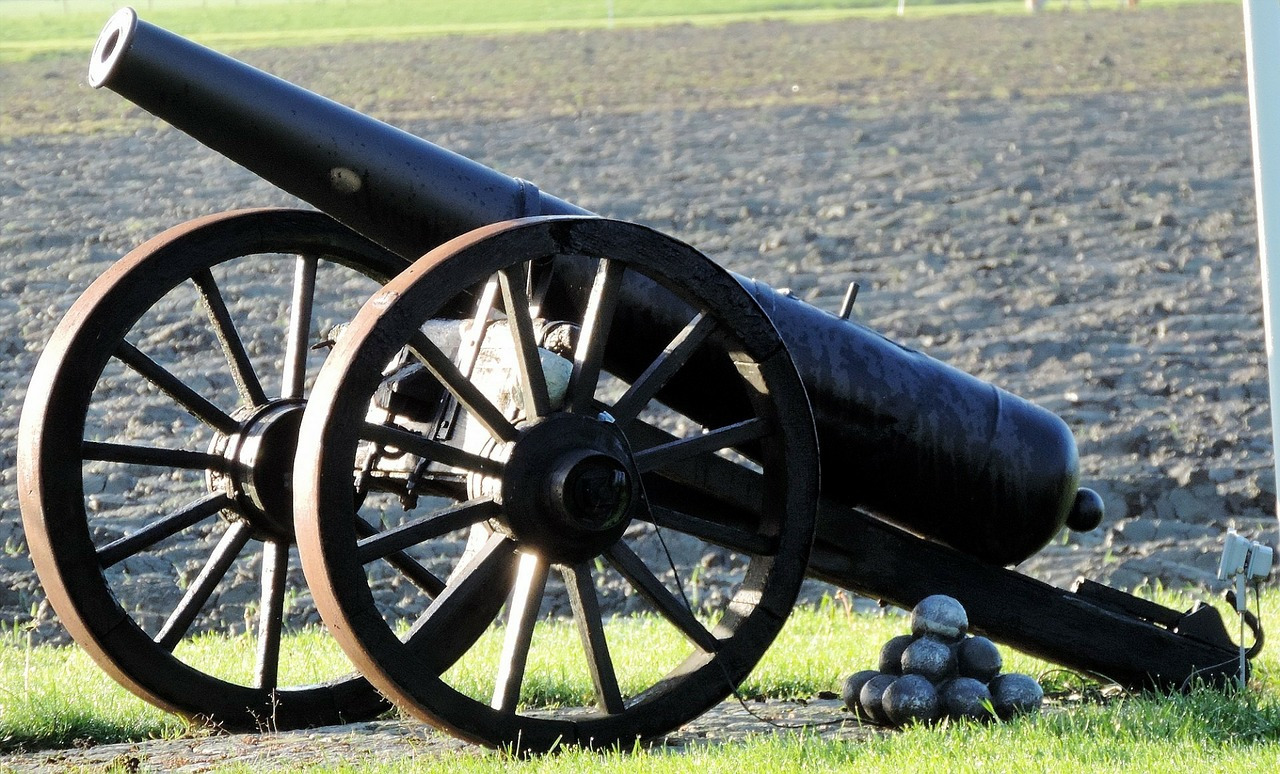
\includegraphics[scale=0.2]{cannon}
    \caption{http://maxpixel.freegreatpicture.com/Cannonballs-Weapon-Cannon-Cannonball-History-War-314498}
  \end{figure}
\end{frame}

\begin{frame}
  \frametitle{Asunciones del programador frágil}
  \begin{itemize}
  \item El cliente \textbf{sabe} lo que quiere
  \item El programador(equipo) \textbf{sabe} cómo construirlo
  \item \textbf{No} ocurren cambios durante el desarrollo
  \end{itemize}
\end{frame}

\begin{frame}
  \frametitle{Asunciones del programador ágil}
  \begin{itemize}
  \item El cliente \textbf{\soutthick{sabe} descubre} lo que quiere
  \item El programador(equipo) \textbf{\soutthick{sabe} descubre} cómo construirlo
  \item \textbf{\soutthick{No}} ocurren cambios durante el desarrollo
  \end{itemize}
\end{frame}

\begin{frame}
  \frametitle{Manifesto}
  \begin{figure}[ht]
    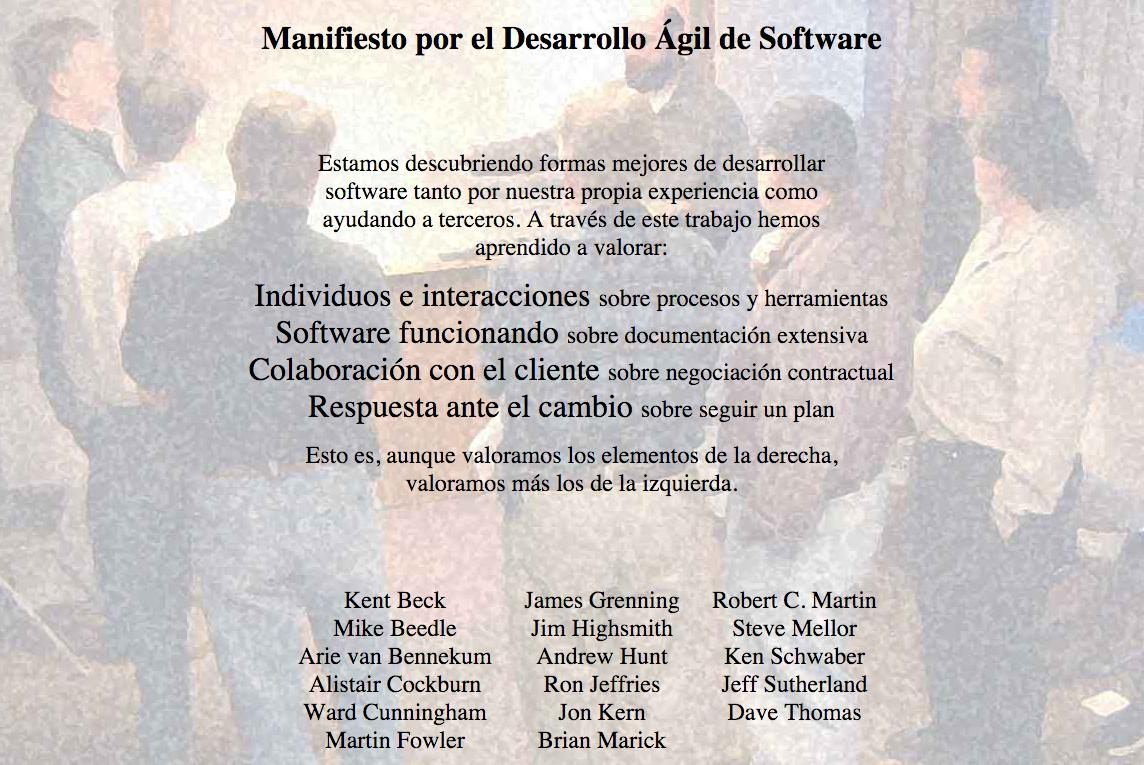
\includegraphics[scale=0.2]{manifesto}
    \caption{http://agilemanifesto.org/}
  \end{figure}
\end{frame}
